\section{Technische Grundlagen} \label{s:basics}
%- Technologische Grundlagen - Grundlagen /
\begin{comment}
TODO:
- im folgenden bezieht sich Client auf MQTT Client
- publishen / subscriben wird zu veröffentlichen / abonnieren
- herausgeber / abonnent wird zu publisher / subscriber
- Thema in Topic umändern

TODO Erklärung zu den einzelnen kapiteln und was sich darin befindet (in den grundlagen)
\end{comment}

\subsection{OSI-Modell} \label{s:osi-model}

\subsection{MQTT} \label{s:mqtt}
%TODO langlebiege connection
\acf{mqtt} wurde ursprünglich von Doktor Andy Stanford-Clark und Arlen Nipper im Jahr 1999 entworfen um Gas- und Ölpiplines zu überwachen. Diese lagen oftmals an entlegenen Orten, wie zum Beispiel auf Übersee, und konnten nicht mit Radiowellen oder einem Kabel zum Festland erreicht werden. Zu dieser Zeit war die einzige Option um Sensordaten auf einen Server zu übertragen eine auf Datendurchsatz abgerechnete Satellitenkommunikation. Bei mehreren tausend Sensoren wurde somit ein Protokoll benötigt, das die Daten zuverlässig mit minimaler Bandbreite an die Server auf dem Festland übermitteln kann.
\ac{mqtt} wurde im Jahr 2013 von der \ac{oasis} als Open Source standatisiert und wird heutzutage von vielen gro{\ss}en \ac{iot} Platformen unterstützt.
%TODO welche ??
\cite{WhatMQTTDefinition}\\
Es gibt derzeit zwei Versionen der MQTT Spezifikation: \verb|3.1.1| und \verb|5|. Alle Referenzen, falls nicht explizit gekennzeichnet, beziehen sich auf die aktuelle Version \verb|5| des Protokolls.\\
\ac{mqtt} ist ein Layer 7 \textit{Publish and Subscribe} Protkoll, das auf \acs{tcp} / \acs{ip} aufsetzt. Anders als das Request / Response Paradigma bei \acs{http} ist \ac{mqtt} Event gesteuert und erlaubt Nachrichten direkt an einen bestimmten Client zu schicken. Somit muss nicht periodisch nach neuen Nachrichten gefragt werden. Zusammen mit einem fixen Paket-Header von nur zwei Byte sorgen diese Eigeschaften für einen geringen Datendurchsatz.\cite{WhatMQTTDefinition}

\subsubsection{Publish and Subscribe} \label{s:publish-subscribe}
%TODO erwähnen das es sich um filter handelt
\ac{mqtt} nutzt das \textit{Publish and Subscribe} Kommunikationsschema, das eine Struktur bietet um Nachrichten zwischen Herausgeber und Abonnent auszutauschen. In diesem Schema gibt es zwei unterschiedliche Systeme:
\begin{itemize}
    \item Clients
    \item Broker
\end{itemize}
Clients sind alle Teilnehmer dieses Systems, die Nachricht empfangen oder veröffentlichen wollen. Diese setzten auf einen Broker als Mittelsmann um die Nachrichten erfolgreich zu vermitteln.\cite{teamGettingStartedMQTT} Jede Nachricht wird durch den Herausgeber in bestimmte Klassen kategorisiert. Der Herausgeber wei{\ss}t nicht ob, oder wer, an dieser Nachricht interessiert ist und schickt die klassifizierte Nachricht an den Broker. Clients, die an bestimmten Nachrichten interessiert sind, müssen bei dem Broker ein Abonnement erstellen und dabei die gewünschte Kategorie angeben. Somit kann der Broker eingehende kategorisierte Nachrichten an die entsprechenden Clients weiterleiten. Der Broker kann Nachrichten zudem auch aufbewahren, sodass Clients, die zu einem späteren Zeitpunkt auf ein Thema abonnieren, ebenfalls die vergangenen Nachrichten erhalten. Durch dieses System entsteht eine Entkopplung der einzelnen Clients auf mehreren Ebenen.\cite{EverythingYouNeed}
\begin{itemize}
    \item \textbf{Räumliche Entkopplung:} Herausgeber und Abonnent der Nachricht müssen sich nicht kennen.
    \item \textbf{Zeitliche Entkopplung:} Herausgeber und Abonnent müssen nicht zur selben Zeit aktiv sein.
    \item \textbf{Synchronisierungs Entkopplung:} Herausgeber und Abonnent müssen ihre Operationen beim publizieren und konsumieren nicht unterbrechen.
%TODO warum?:
\end{itemize}
\cite{teamPublishSubscribeMQTT}
In verteilten System, wo einzelne Komponenten oftmals sehr unterschiedlich sind, spielt ein solches Konzept eine gro{\ss}e Rolle, da es eine einheitliche Abstraktion der Kommunikationsebene bietet.\cite{domingusDistributedSystemsIntroduction2020}
% TODO mehr zu distributed systems
% TODO bild publisher - subscriber topic
% TODO bild von sensoren / broker / downstream clients
\begin{figure}
    \centering
    %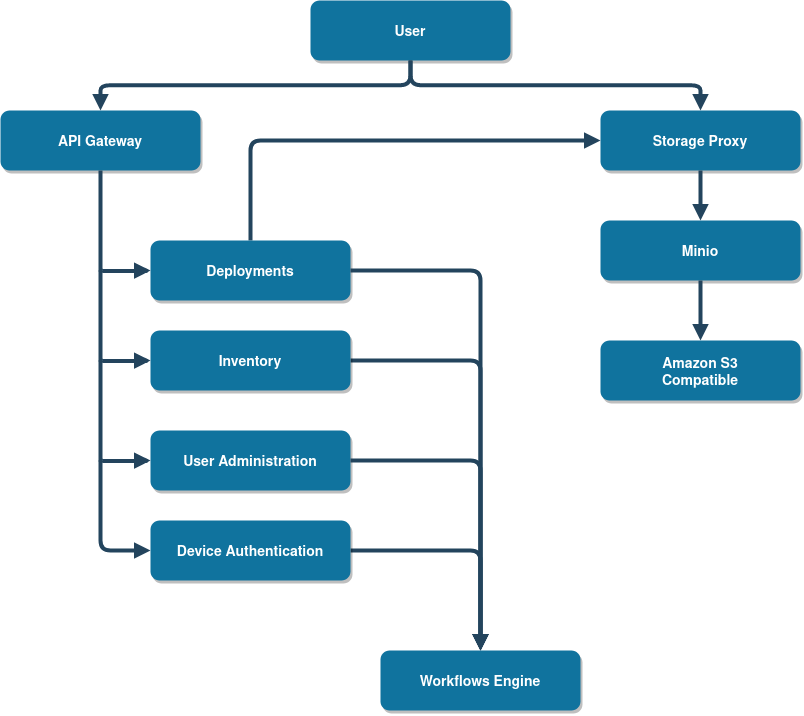
\includegraphics[scale=0.5]{images/integration-app.png}
    \caption{Publish and Subscribe Architektur basirend auf Themen}
    \label{fig:publish-subscribe}
\end{figure}
Im Kontext \ac{mqtt} werden Nachrichten in eine hieraschich aufgebaute Themenstruktur klassifiziert. Themen werden mit einem Schrägstrich (\verb|/|) getrennt und sehen zum Beispiel wie folgt aus: \verb|sensors/temperature/celcius|. Abbildung \ref{fig:publish-subscribe} zeigt einen Client, der auf das Thema \verb|bla| Nachrichten veröffentlicht. Diese wird an zwei weitere Clients durch den Broker weitergeleitet, da diese das Thema \verb|bla| abonniert haben. Themen müssen auf einem Broker nicht explizit angelegt werden. Sobald ein Client auf einem Thema publiziert oder es abonniert, wird dieses automatisch angelegt.\cite{WhatMQTTDefinition}\\
Beim abonnieren eines Themas kann entweder ein spezifisches Thema oder eine Kombination aus Thema und Wildcard verwendet werden. Bei einer Wildcard werden zwischen den folgenden zwei unterschieden:\cite{mqtt5Specification}
\begin{itemize}
    \item Multi-level '\verb|#|': Schlie{\ss}t das Vorgänger- und alle nachfolgenden Themen mit ein.
    \item Single-level '\verb|+|': Schlie{\ss}t alle Themen auf einer einzigen Ebene mit ein.
\end{itemize}
Bei der folgenden Themenstruktur
\begin{itemize}
    \item \verb|sensors|
    \item \verb|sensors/temperature|
    \item \verb|sensors/temperature/celcius|
    \item \verb|sensors/temperature/kelvin|
    \item \verb|sensors/fuel|
    \item \verb|sensors/fuel/tank1|
    \item \verb|sensors/fuel/tank2|
\end{itemize}
schlie{\ss}t ein Abonnement auf \verb|sensors/#| alle Themen mit ein. Bei einem Abonnement auf \verb|sensors/+| sind hingegen nur diese Themen mit eingeschlossen:
\begin{itemize}
    \item \verb|sensors/temperature|
    \item \verb|sensors/fuel|
\end{itemize}

\subsubsection{Quality of Service} \label{s:qos}
Je zuverlässiger eine Nachricht übermittelt werden soll, desto mehr Datendurchsatz verursacht diese Nachricht im gesamten System. Wenn ein Client wissen will, ob seine Nachricht im Broker eingetroffen ist, muss der Broker dem Client eine entsprechende Rückmeldung geben. Andernfalls kann der Client seine Nachricht an den Broker schicken ohne eine Rückmeldung zu erwarten. Dies ist vergleichsweise im \ac{http} nicht möglicht. Dort muss auf jede Nachricht geantwortet werden.\\
Bei \ac{mqtt} wird die Zuverlässigkeit der Übermittlung einer Nachricht mit einem \textit{\acf{qos}} Level festgelegt. Eine Nachricht publizierte Nachricht muss einen der drei \ac{qos} Level haben:
\begin{itemize}
    \item \ac{qos} 0: Maximal eine Zustellung der Nachricht.
    \item \ac{qos} 1: Mindestens eine Zustellung der Nachricht.
    \item \ac{qos} 2: Genau eine Zustellung der Nachricht.
\end{itemize}
Bei \ac{qos} Level 1 und 2 werden Handshakes zur Verifizierung der Paketübermittelung eingesetzt.\cite{mqtt5Specification}

\subsubsection{Retained Message} \label{s:retained-messages}
In \ac{mqtt} kann pro Topic die letzte veröffentlichte Nachricht aufbewahrt werden.
Dazu muss im \verb|PUBLISH| Paket die \verb|RETAIN| Kennzeichnung gesetzt werden.
In diesem Fall speichert der Broker die Nachricht mit dem dazugehörigen Topic und \ac{qos} Level ab.
Falls bereits eine Aufbewahrte Nachricht (engl. \textit(Retained Message)) auf diesem Topic vorhanden ist, wird sie überschrieben.
Jeder Client, der ein Topic abonniert das eine Retained Message besitzt, bekommt diese Nachricht direkt nach dem abonnieren zugeschickt.
Dies trifft auch zu, falls das Topic mit der Retained Message durch einen Wildcard Filter abonniert wurde.
\cite{teamRetainedMessagesMQTT}
Um eine Retained Message zu löschen muss eine neue Nachricht auf dem Topic veröffentlicht werden mit der \verb|RETAIN| Kennzeichnung und einem leeren Payload. Der Broker löscht die aktuelle Retained Message und neue Subscriber werden erst Nachrichten von diesem Topic erhalten, sobald eine neue Nachricht dort veröffentlich wird.
% TODO zeitliche zeichnung mit mehreren clients und subscribe events
Falls ein Topic eine Retained Message (folglich \textit{M1} genannt) besitzt und eine neue Nachricht ohne \verb|RETAIN| Kennzeichnung auf diesem Topic veröffentlicht wird, überschreibt diese nicht die aktuelle Retained Message. Neue Subscriber erhalten weiterhin die Nachricht \textit{M1}.
%TODO zeichnung!
\cite{mqtt5Specification}
\\
Retained Messages helfen neuen Subscribern direkt einen Wert zu kriegen nachdem sie ein Topic abonniert haben. Eine Retained Messaged wird auch \textit{last known good value} genannt.
\cite{teamRetainedMessagesMQTT}
Als Beispiel dient ein Temperatursensor, der alle zehn Minuten seine Temperatur auf das Topic \verb|sensors/temperature| veröffentlicht. Um den aktuellen Temperaturwert abzufragen gibt es ein Konsolenprogramm, das bei der Ausführung eine Verbindung zu dem Broker herstellt, das Topic \verb|sensors/temperature| abonniert, den ersten erhaltenen Wert auf der Konsole ausgibt, das Topic deabonniert und die Verbindung wieder schlie{\ss}t. Wenn das Programm eine Minute nachdem der Temperatursensor seine Nachricht veröffentlicht hat ausgeführt wird, muss der Benutzer neun Minuten warten bis er die aktuelle Temperatur angezeigt bekommt. Wenn der Temperatursensor seine Nachrichten hingegen als Retained Message veröffentlicht, bekommt das Konsolenprogramm nach dem abonnieren den letzten Temperaturwert und kann diesen anzeigen.

\subsubsection{Paket Struktur} \label{s:packet-structure}
\ac{mqtt} hat die Absicht ein leichtgewichtiges Protokoll zu sein. Tabelle \ref{table:mqtt-packet-structure} zeigt den Aufbau eines jeden \ac{mqtt} Paketes. Die fixe Kopfzeile ist zwei Byte gro{\ss} und muss in jedem Paket vorhanden sein. Basierend auf der Art des Paketes, das in der fixen Kopfzeile angegeben wird, sind zusätzlich eine variable Kopfzeile und weitere Daten möglich.\cite{mqtt5Specification}
\begin{table}[h!]
\centering
\renewcommand{\arraystretch}{1.5}
\begin{tabular}{|c|}
    \hline
    Fixe Kopfzeile, muss in jedem \ac{mqtt} Paket vorhanden sein \\
    \hline
    Variable Kopfzeile, optional \\
    \hline
    Daten des Pakets, optional \\
    \hline
\end{tabular}
\caption{Struktur eines \ac{mqtt} Paketes}
\label{table:mqtt-packet-structure}
\end{table}
Tabelle \ref{table:fixed-header} zeigt den detaillierten Aufbau der fixen Kopfzeile. Im ersten Byte werden Bit sieben bis vier für die spezifische Art des Paketes verwendet. Tabelle \ref{table:mqtt-packet-types} enhält eine Liste mit allen möglichen Pakettypen und deren Wert. Byte zwei gibt die restliche Paketlänge enkodiert als \textit{Variable Byte Integer} an. Die Restliche Paketlänge setzt sich aus ... zusammen. Ein \textit{Variable Byte Integer} ist ... . Die maximale Paketgrö{\ss}e beträgt ... .\cite{mqtt5Specification}
% TODO was ist ein variable byte integer
% TODO wie setzt sich die restliche paketlänge zusammen
\begin{table}[h!]
\centering
\renewcommand{\arraystretch}{1.5}
\begin{tabularx}{\textwidth}{|l| *{8}{Y|}}
    \hline
    Bit & 7 & 6 & 5 & 4 & 3 & 2 & 1 & 0 \\
    \hline
    \hline
    Byte 1 & \multicolumn{4}{c|}{\ac{mqtt} Paketart} & \multicolumn{4}{c|}{Paketart spezifische Kennzeichnung} \\
    \hline
    Byte 2 & \multicolumn{8}{c|}{Restliche Paketlänge} \\
    \hline
\end{tabularx}
\caption{Aufbau der fixen \ac{mqtt} Kopfzeile}
\label{table:fixed-header}
\end{table}

\begin{table}[h!]
\centering
\renewcommand{\arraystretch}{1.5}
\begin{tabular}{|l|c|}
    \hline
    \textbf{Name} & \textbf{Wert} \\
    \hline
    \hline
    Reserved & 0 \\
    \hline
    CONNECT & 1 \\
    \hline
    CONNACK & 2 \\
    \hline
    PUBLISH & 3 \\
    \hline
    PUBACK & 4 \\
    \hline
    PUBREC & 5 \\
    \hline
    PUBREL & 6 \\
    \hline
    PUBCOMP & 7 \\
    \hline
    SUBSCRIBE & 8 \\
    \hline
    SUBACK & 9 \\
    \hline
    UNSUBSCRIBE & 10 \\
    \hline
    UNSUBACK & 11 \\
    \hline
    PINGREQ & 12 \\
    \hline
    PINGRESP & 13 \\
    \hline
    DISCONNECT & 14 \\
    \hline
    AUTH & 15 \\
    \hline
\end{tabular}
\caption{Verfügbare \ac{mqtt} Paketarten und deren Wert}
\label{table:mqtt-packet-types}
\end{table}

\subsubsection{MQTT CONNECT} \label{s:mqtt-connect}
Nachdem eine Netzwerkverbindung zwischen einen Client und einem Broker aufgebaut wurde, muss das erste Paket eines Clients ein \verb|CONNECT| Paket sein. Tabelle \ref{table:mqtt-connect-packet-variable-header} zeigt den Aufbau und Inhalt einer Beispielhaften variablen Kopfzeile eines \verb|CONNECT| Paketes. Die ersten sechs Byte geben den Namen es Protokolls als UTF-8 encodierten String an. Dieser wird sich in zukünftigen Versionen nicht ändern und dient als Identifikationsmerkmal des \ac{mqtt} Protokolls für Server, die mehrere Protokolle implementiert haben. Byte sieben gibt die verwendete \ac{mqtt} Version des Clients an. In Byte acht kann der Client Kennzeichnungen für die Präsenz der optionalen Daten setzen. Die Länge der Eigenschaften wird mit Byte elf bestimmt. In den Eigenschaften kann der Client zum Beispiel eine maximale Paketgrö{\ss}e oder Themen Aliasse setzen.\cite{mqtt5Specification}\\
Nach der variablen Kopfzeile folgen die Daten (Payload) des \verb|CONNECT| Paketes. Diese sind eine oder mehrere Felder mit ihrer Länge als Präfix. Byte acht der variablen Kopfzeile bestimmt das Vorkommen der Felder, die - falls vorhanden - eine strikte Reihenfolge einhalten müssen.
\begin{enumerate}
    \item Client Idenfikationsnummer
    \item \textit{Will} Eigenschaften
    \item \textit{Will} Thema
    \item \textit{Will} Daten (Payload)
    \item Benutzername
    \item Passwort
\end{enumerate}
Die Client Identifikationsnummer ist als einziges Feld nicht optional. Sie muss ein UTF-8 enkodierter String aus folgenden Zeichen sein:
\begin{itemize}
    \item 0-9
    \item a-z
    \item A-Z
\end{itemize}
Eine Client Identifikationsnummer dient zur Identifikation des aktuellen Zustands des Clients und muss daher einzigartig vergeben sein. Ist bereits ein Client mit der gleich Identifikationsnummer an dem Broker verbunden, wird die Verbindung des existierenden Clients getrennt und es findet ein \textit{Client takeover} statt (siehe \ref{s:client-takeover}).\cite{mqtt5Specification}
%TODO auch die anderen optionalen daten erklären?
\begin{table}[h!]
\centering
\renewcommand{\arraystretch}{1.5}
\begin{tabularx}{\textwidth}{|l|l|c| *{8}{Y|}}
    \hline
    & \textbf{Beschreibung} & \textbf{Wert} &
      \textbf{7} & \textbf{6} & \textbf{5} &
      \textbf{4} & \textbf{3} & \textbf{2} &
      \textbf{1} & \textbf{0} \\
    \hline
    \hline
    Byte 1 & Länge \acs{msb} & 0 & 0 & 0 & 0 & 0 & 0 & 0 & 0 & 0 \\
    \hline
    Byte 2 & Länge \acs{lsb} & 4 & 0 & 0 & 0 & 0 & 0 & 1 & 0 & 0 \\
    \hline
    Byte 3 & UTF-8 Char & 'M' & 0 & 1 & 0 & 0 & 1 & 1 & 0 & 1 \\
    \hline
    Byte 4 & UTF-8 Char & 'Q' & 0 & 1 & 0 & 1 & 0 & 0 & 0 & 1 \\
    \hline
    Byte 5 & UTF-8 Char & 'T' & 0 & 1 & 0 & 1 & 0 & 1 & 0 & 0 \\
    \hline
    Byte 6 & UTF-8 Char & 'T' & 0 & 1 & 0 & 1 & 0 & 1 & 0 & 0 \\
    \hline
    Byte 7 & Protokoll Version & 5 & 0 & 0 & 0 & 0 & 0 & 1 & 0 & 1 \\
    \hline
    Byte 8 &
        \makecell[l]{Benutzername Kennzeichnung \\ Passwort Kennzeichnung \\ \textit{Will} speichern \\ \textit{Will} \ac{qos} Level \\ \textit{Will} Kennzeichnung \\ Frische Session \\ Reserviert} &
        \makecell{1 \\ 1 \\ 0 \\ 01 \\ 1 \\ 1 \\ 0} &
        1 & 1 & 0 & 0 & 1 & 1 & 1 & 0 \\
    \hline
    Byte 9 & Keep Alive \acs{msb} & 0 & 0 & 0 & 0 & 0 & 0 & 0 & 0 & 0 \\
    \hline
    Byte 10 & Keep Alive \acs{lsb} & 10 & 0 & 0 & 0 & 0 & 1 & 0 & 1 & 0 \\
    \hline
    Byte 11 & Länge der Eigenschaften & 0 & 0 & 0 & 0 & 0 & 0 & 0 & 0 & 0 \\
    \hline
\end{tabularx}
\caption{Beispielhaftes \ac{mqtt} CONNECT Paket}
\label{table:mqtt-connect-packet-variable-header}
\end{table}
Der Broker muss eine \verb|CONNECT| Nachricht von einem Client mit einem \verb|CONNACK| Paket beantworten.\cite{mqtt5Specification}

\subsubsection{Last Will Nachricht} \label{s:last-will}
Ein Client kann bei der Verbindung zu einem Broker einen letzten Willen (engl. \textit{Last Will}) als Nachricht definieren. Diese Nachricht wird auf ein ebenfalls angegebenes Topic veröffentlich sobald die Verbindung zum Client unterbricht und dieser nicht in einer definierten Zeit seine Verbindung zum Broker wieder aufbauen kann. Falls der Client seine Verbindung Protokollkonform beendet, wird die Last Will Nachricht nicht veröffentlicht.
\cite{soniSURVEYMQTTPROTOCOL}\\
Die Last Will Nachricht kann in Sicherheitsrelevanten Applikationen eingesetzt werden. Als Beispiel dient ein Bewegungssensor der eine Eingangtür überwachen soll. Falls dieser Sensor vor einem Einbruch mutwillig zerstört wird, verliert dieser die Verbindung zum Broker und seine Last Will Nachricht wird veröffentlicht. Somit kann ein System auch auf ungeplante Events reagieren.

\subsubsection{Shared Subscriptions} \label{s:shared-subsriptions}
In \ac{mqtt} Version 5 wurden \textit{Shared Subscriptions} eingeführt, die es Clients erlauben ein Abonnement untereinander zu teilen. Diese Clients werden in eine \textit{Shared Subscription Group} zusammengefasst. Bei einem normalen Abonnement erhält jeder Client, der das gleiche Thema abonniert hat, eine Kopie der Nachricht. Bei einer \textit{Shared Subscription} erhält immer nur ein Client der \textit{Shared Subscription Group} die Nachricht in abwechselnder Reihenfolge. Dieser Mechanismus wird auch als \textit{Client Load Balancing} bezeichnet, da die Last eines Themas auf mehrere Abonnenten verteilt wird.\cite{raschbichlerMQTTHowNew}
Shared Subscriptions verwenden Standard \ac{mqtt} Mechanismen. Jeder Client kann Teil einer Shared Subscription Group werden, indem er diese Topic Struktur einhält: \verb|$share/GROUPID/TOPIC|.
\begin{itemize}
    \item \verb|$share|: Statische Shared Subscription Identifikation.
    \item \verb|GROUPID|: Identifikation einer Shared Subscription Group. Darf \verb|/|, \verb|#| und \verb|+| nicht enthalten.
    \item \verb|TOPIC|: Das zu abonnierende Topic.
\end{itemize}
Ein konkretes Beispiel für das abonnieren einer Shared Subscription ist: \verb|$share/group1/sensors/temperature|.
% TODO bild einer shared subscription group

\newpage

\subsection{HiveMQ Broker} \label{s:hivemq-broker}
%TODO write that chapter
Der HiveMQ Broker ist ein Java basierter \ac{mqtt} Broker, der sich auf das Anwendungsfall \acl{iot} spezialisiert.
Er unterstützt alle Versionen des \ac{mqtt} Protokolls und ist Clusterfähig.
HiveMQ Broker ist erweiterbar mit Extensions.

\subsubsection{HiveMQ Cluster} \label{s:hivemq-cluster}
Ein Merkmal des HiveMQ Broker ist die Möglichkeit ein Broker Cluster zu bilden.
Ein Broker Cluster (folgend Cluster genannt) ist ein verteiltes System in welchem sich mehrere HiveMQ Broker zusammenschlie{\ss}en.
Ein Cluster bildet für Clients eine einzige logische Einheit.
Dies bedeutet, für einen Client macht es keinen Unterschied ob er zu einem einzigen HiveMQ Broker oder zu einem Cluster verbunden ist.
\cite{HiveMQClusterHiveMQ}
Durch das clustern der HiveMQ Broker ensteht eine horizontale Skalierung. Wie in Kapitel \ref{s:domain} anwendungsdomäne bereits erläutert, kann der Anwendungsfall \ac{iot} zu mehreren Millionen Clients führen wobei eine vertikale Skalierung an ihre Grenzen sto{\ss}en kann.
%TODO erkären warum an die grenzen sto{\ss}en?
\begin{itemize}
    \item \textbf{Vertikale Skalierung:} Fügt mehr Rechen- oder Speichereinheiten zu einem Server hinzu.
    \item \textbf{Horizontale Skalierung:} Fügt mehrere Server zu einer logischen Recheneinheit hinzu. Dabei kann die Arbeitslast auf die einzelnen Server verteilt werden.
\end{itemize}
%TODO bessere quelle für skalierung?
\cite{HowScaleIT}

Ein HiveMQ Broker in einem HiveMQ Cluster wird als ein HiveMQ Node (folgend Node genannt) bezeichnet.
Damit sich mehrere Nodes zu einem Cluster zusammenschlie{\ss}en muss jeder Node:
\begin{itemize}
    \item ein HiveMQ Enterprise Broker sein.
    \item die anderen Nodes über ein Netzwerk erreichen können.
    \item das \textit{clustering} in seiner Konfiguration eingeschaltet haben.
    \item die anderen Nodes mit der \textit{Cluster Discovery} auffinden können.
\end{itemize}
Die Cluster Discovery beschreibt den Mechanismus wie sich individuelle Nodes gegenseitig finden können um ein Cluster zu bilden. Es stehen folgende Möglichkeiten zur Verfügung:
\begin{itemize}
    \item \textbf{static:} Jeder Node wird mit einer statischen Liste von allen Nodes und deren \ac{ip} Adresse / Port provisioniert.
    \item \textbf{multicast:} Nodes finden dynamisch andere Nodes, die die selbe multicast Adresse und Port benutzen.
    \item \textbf{broadcast:} Nodes finden dynamisch andere Nodes im selben Subnetzwerk indem sie die Broadcast \ac{ip} Adresse benutzen.
    \item \textbf{extension:} Es kann eine HiveMQ Erweiterung benutzt werden um andere Nodes zu entdecken.
    \item \textbf{dns extension:} Nodes finden dynamisch andere Nodes über einen \textit{round-robin} \acs{dns} A record.
\end{itemize}
HiveMQ ist in der Lage die Clustergrö{\ss}e zur Laufzeit dynamisch anzupassen. Diesen Mechanismus muss der gewählte Cluster Discovery Modus jedoch unterstützten.
\cite{HiveMQClusterHiveMQ}

\subsubsubsection{Overload Protection} \label{sb:overload-protection}
HiveMQ stellt einen eingebauten Überlastschutz (engl. \textit{Overload Protection}) für ein HiveMQ Cluster bereit. Jeder Node eines Cluster ist in der Lage die Rate der eingehenden Nachrichten zu reduzieren. Dieser Mechanismus erhöht die Stabilität des Cluster indem gezielt Clients, die zu einer Überlast beitragen, gedrosselt werden. Dadurch kann sich das Cluster von einer Überlastsituation erholen ohne die Service Qualität für alle Clients zu reduzieren.
Jeder Node eines Clusters berechnet durchgehend einen individuellen \textit{Overload Protection Level} auf Basis der Menge aller:
\begin{itemize}
    \item eingehenden \verb|PUBLISH| Nachrichten
    \item Retained Messages
    \item verbundenen Clients
    \item Queued Messages
\end{itemize}
% TODO explain queued messages
Das drosseln von Clients basiert auf einem Credit System. Jeder Client erhält nach dem Aufbau einer Verbindung ein Guthaben von 50,000 Credits. Um auf einem Topic Nachrichten zu veröffentlichen muss ein Client mit seinen Credits bezahlen. Diese werden alle 200 Millisekunden um einen bestimmten Wert regeniert bis das maximale Guthaben von 50,000 erreicht wurde. Dieser Wert richtet sich nach dem derzeitigen Overload Protection Level des Nodes, auf dem der Client verbunden ist.
% TODO ist es wirklich der Node ? oder ist es der Node auf dem das Topic liegt?
Hat ein Client alle seine Credits verbraucht, wird \ac{tcp} Backpressure auf dem Socket des Clients angewandt und dieser kann keine Nachrichten mehr veröffentlichen.
Ist der Zeitraum, in dem \ac{tcp} Backpressure für einen Client angewandt wird, länger als der konfigurierte Keep-Alive Wert, wird die Verbindung des Clients unterbrochen.
Neben \ac{mqtt} Clients kann auch eine Topologieänderung des Clusters zu einer Erhöhung des Overload Protection Levels führen.
\cite{ClusterOverloadProtection}

\subsubsubsection{Client Queue}
\subsubsubsection{Replication}

\subsubsection{Persistente Session} \label{s:persistent-session}
Um Nachrichten von einem \ac{mqtt} Broker zu erhalten, muss sich ein Client zu diesem verbinden und eine Subscription auf ein Topic erstellen.
Jedes mal wenn die Verbindung zum Client unterbrochen wird, müssen die Verbindung und alle Subscriptions neu aufgebaut werden.
Für einen Client mit limitierten Ressourcen ist dies eine Belastung.
Um diese Belastung zu reduzieren kann der Client beim Aufbau der Verbindung eine persistente Session anfordern, indem dieser Bit eins von Byte acht des variablen Header der \verb|CONNECT| Nachricht (siehe Tabelle \ref{table:mqtt-connect-packet-variable-header}) auf null setzt.
Ist dieses Bit hingegen auf eins gesetzt, werden alle Nachrichten und Informationen von vorherigen Sessions gelöscht.
Eine persistente Session speichert folgende Daten auf dem Broker:
\begin{itemize}
    \item Die Existenz einer persistenten Session. Als Identifikation wird die \acs{clientid} verwendet.
    \item Alle Subscriptions des Clients.
    \item Alle Nachrichten mit einem \ac{qos} Level eins oder zwei, die der Client noch nicht bestätigt hat.
    \item Alle Nachrichten mit einem \ac{qos} Level eins oder zwei, die der Client aufgrund der unterbrochenen Verbindung nicht erhalten konnte.
    \item Alle Nachrichten mit einem \ac{qos} Level zwei, die der Client veröffentlicht hat und noch nicht bestätigt wurden.
\end{itemize}
Neben dem Broker muss ein Client auch Informationen bei einer persistenten Session speichern. Er ist verantwortlich die folgenden Daten zu persistieren:
\begin{itemize}
    \item Seine eigene \ac{clientid}. Diese wird als Identifikationsmerkmal einer persistenten Session auf dem Broker genutzt und muss bei einer erneuten Verbindung immer gleich sein.
    \item Alle \ac{qos} Level eins oder zwei Nachrichten, die noch nicht vom Broker bestätigt wurden.
    \item Alle \ac{qos} Level zwei Nachrichten, die der Client vom Broker erhalten hat und noch nicht vollständig bestätigt wurden.
\end{itemize}
Sobald ein Client die Verbindung zu einem Broker verliert und eine persistente Session aktiv ist, versucht der Broker die Daten des Clients solange wie möglich zu persistieren bis dieser sich erneut verbindet. Falls der Broker während der Zeit, die der Client nicht verbunden ist, keinen verfügbaren Arbeitsspeicher mehr hat, besteht die Möglichkeit, dass die persistente Session vom Broker gelöscht wird.
\cite{teamPersistentSessionQueuing}

\subsubsubsection{Client Takeover} \label{s:client-takeover}
Wie bereits im Kapitel \ref{s:persistent-session} beschrieben kann ein Client eine persistente Session bei einem Broker anfordern. Dabei werden zum Beispiel Nachrichten mit einem \ac{qos} Level von eins oder zwei auf dem Broker nachgehalten, falls der Client seine Verbindung verliert. Ein Client Takeover findet statt, wenn der Broker eine neue Client Verbindung erhält aber noch eine offene Verbindung mit der selben \ac{clientid} hat. Dies kann bei \textit{halb-offenen \acs{tcp} Verbindungen} vorkommen, die, wie Andy Stanford-Clark beschreibt, auch bei \ac{tcp} auftreten können:
"Although TCP/IP in theory notifies you when a socket breaks, in practice, particularly on things like mobile and satellite links, which often 'fake' TCP over the air and put headers back on at each end, it’s quite possible for a TCP session to 'black hole', i.e. it appears to be open still, but in fact is just dumping anything you write to it onto the floor."
% TODO quelle: https://groups.google.com/forum/#!msg/mqtt/zRqd8JbY4oM/XrMwlQ5TU0EJ
Der Broker beendet die existierende Verbindung und assoziiert die persistente Session - falls vorhanden - nun mit dem neuen Client.
\cite{teamKeepAliveClient}
%TODO where to quote?

\subsection{Load Balancing} \label{s:load-balancing}
%TODO Beispiel Web-Applikation
Um Applikationen auf einem Server bereitzustellen muss man einen geeigneten Server suchen. In diesem Prozess testet man die Applikation wie viel \acs{cpu}, \acs{ram} und Speicherplatz diese in einer Produktivumgebung benötigt. Wenn nun mehr Leute als erwartet die Applikation benutzen braucht diese mehr Recheneinheiten um die neue Arbeitslast abzuarbeiten. Eine Möglichkeit ist, den Server herunterzufahren, ihm mehr \acs{cpu} und \acs{ram} zu geben und ihn wieder zu starten. Dieser Prozess wird auch vertikale Skalierung genannt und hat Grenzen.\cite{bourkeServerLoadBalancing2001}
Als Beispiel für diese Grenze ist der Rechenleistungsstärkste Server, den man zurzeit bei Amazon AWS mieten kann, mit 96 virtuellen \acs{cpu} Kernen und 375 Gigabyte \acs{ram}.\cite{EC2OnDemandInstance}
Es gibt mehrere Gründe wann eine vertikale Skalierung an ihre Grenzen stö{\ss}t:
\begin{itemize}
    \item Der Server ist nicht mehr erweiterbar an \acs{cpu}, \acs{ram} oder Speicherplatz.
    \item Ein neustarten des Servers um eine vertikale Skalierung durchzuführen ist nicht möglich.
\end{itemize}
\cite{bourkeServerLoadBalancing2001}
Die alternative zu einer vertikalen Skalierung ist die horizontale Skalierung. Bei einer horizontalen Skalierung werden nicht die Kapazitäten des Servers erhöht, sondern es werden weitere Server bereitgestellt.
Wird Beispielweise ein \acs{http} Web-Server, der auf jeden Request ein \verb|"Hello World"| zurückgibt, auf einem Server bereitgestellt, der zwei \ac{cpu} Kerne und zwei Gigabyte \ac{ram} hat, sieht eine Skalierung wie folgt aus:
\begin{itemize}
    \item \textbf{Vertikale Skalierung:} Es werden vier \ac{cpu} Kerne und vier Gigabyte \ac{ram} zu dem Server hinzugefügt.
    \item \textbf{Horizontale Skalierung:} Es wird ein weiterer unabhängiger Server mit der Web-Applikation bereitgestellt, der die Requests bearbeiten kann.
\end{itemize}
Nicht jede Applikation ist für eine horizontale Applikation geeignet. Würde der Web-Server einen internen Zähler an den Benutzer zurückgeben, wie viele Requests der Server bereits abgearbeitet hat, müsste die Applikation diesen Zähler mit allen anderen Servern die an der horizontalen Skalierung teilnehmen teilen.
Ein weiteres Problem ist die Bereitstellung der horizontalen Server. Der Endnutzer der Web-Applikation muss die \ac{ip} Adressen aller Server kennen um auf diese zuzugreifen.
% TODO cite horizontale und vertikale skalierung
% TODO verschiedenen LB Algorithmen
% least connection
% round robin

\subsubsection{Load Balancing Algorithmen}
% TODO vielleicht keine ganzen kapitel

\subsubsubsection{DNS Round Robin} \label{s:dns-round-robin}
% TODO link hivemq dns extension with this chapter
Um die \ac{ip} Adressen aller Teilnehmer einer horzontalen Skalierung einem Endnutzer mitzuteilen wurde das \ac{dns} A Eintrag Round Robin Load Balancing entwickelt. Bei einen \ac{dns} A Eintrag muss eine \ac{ip}v4 Adresse hinterlegt werden. Bei einem \ac{dns} Round Robin können mehrere \ac{ip}v4 Adressen bei einer Domain hinterlegt werden, sodass ein Endnutzer nur den Domainnamen kennen muss und alle Teilnehmer einer horizontalen Skalierung erreichen kann.

Literatur zu der Limitierung von \ac{dns} A Round Robin findet sich im Buch Server Load Balancing von Tony Bourke.\cite{bourkeServerLoadBalancing2001}

\subsubsubsection{Round Robin}
\subsubsubsection{Weighted Round Robin}
\subsubsubsection{Least Connection}

\subsubsection{Server Load Balancing}
Ein Load Balancer ist ein Gerät, das Traffic auf verschiedene Maschinen verteilt. Dies hat den Effekt, das mehrere Maschinen als Eine erscheinen.
\cite{bourkeServerLoadBalancing2001}

\subsubsection{Envoy} \label{s:envoy}
Envoy ist ein Layer drei/vier Netzwerk Proxy und ist für gro{\ss}e moderne Service orientierte Architekturen entworfen worden. Um dies zu erreichen stellt Envoy folgende abstrakte Features bereit:
\begin{itemize}
    \item \textbf{Layer 3/4 Filter:} Envoy erlaubt das dazuschalten von \acs{tcp} oder \acs{udp} Filtern in die Netzwerk Pipeline.
    \item \textbf{\acs{http} Layer 7 Filter:} \acs{http} Filter können über einen HTTP Connection Manager hinzugefügt werden. Filter wie \textit{buffering}, \textit{routing} und \textit{rate-limiting} sind bereits in Envoy integriert.
    \item \textbf{Dynamische Konfiguration:} Envoy kann dynamisch über eine \textit{Data-Plane API} provisioniert werden.
    \item \textbf{:}
    \item \textbf{:}
    \item \textbf{:}
\end{itemize}
\cite{WhatEnvoyEnvoy}

\subsubsubsection{Hot Restart}
\subsubsubsection{Data-Plane API}
